\documentclass[10pt, aspectratio=169]{beamer} % Proporción 16:9 para pantallas modernas

% --- Configuración de Idioma y Fuentes ---
\usepackage[utf8]{inputenc}
\usepackage[spanish]{babel}
\usepackage{helvet} % Fuente similar a Arial para mejor lectura
\usepackage{tikz}
\usepackage{graphicx}
\usetikzlibrary{positioning, arrows.meta}

% --- Configuración del Tema Beamer ---
\usetheme{Madrid}
\usecolortheme{whale} % Base azul

% Personalización de colores UCU (Azul institucional)
\definecolor{UCUBlue}{RGB}{0, 74, 153} 
\setbeamercolor{palette primary}{bg=UCUBlue, fg=white}
\setbeamercolor{palette secondary}{bg=UCUBlue!80, fg=white}
\setbeamercolor{palette tertiary}{bg=UCUBlue!60, fg=white}
\setbeamercolor{titlelike}{parent=palette primary}
\setbeamercolor{structure}{fg=UCUBlue}

% --- Paquetes para Código ---
\usepackage{listings}
\definecolor{codegray}{rgb}{0.5,0.5,0.5}
\definecolor{codeblue}{rgb}{0.0, 0.0, 0.8}

\lstset{
    language=C,
    basicstyle=\ttfamily,
    keywordstyle=\color{codeblue},
    commentstyle=\color{codegray},
    numbers=left,
    numberstyle=\tiny,
    breaklines=true,
    frame=single,
    showstringspaces=false
}

% --- Datos de la Presentación ---
\title[Lab 3: FreeRTOS]{Laboratorio 3: FreeRTOS}
\subtitle{Diseño de IoT y Sistemas Embebidos - UCU 2026}
\author[Saucedo et al.]{
Santiago Blanco \\
\and Felipe Paladino \\
\and Piero Saucedo
}
\institute[FIT - UCU]{
    Facultad de Ingeniería y Tecnologías\\
    Universidad Católica del Uruguay
}
\date{28 de mayo de 2026}

% Logo opcional en las esquinas
\titlegraphic{
\includegraphics[width=2cm]{uculogo.png}} % Sube este archivo a tu proyecto

% --- INICIO DEL DOCUMENTO ---
\begin{document}

% Slide de Título
\begin{frame}
    \titlepage
\end{frame}

% Tabla de Contenidos
\begin{frame}{Estructura de la Presentación}
    \tableofcontents
\end{frame}

% --- SECCIÓN: ARQUITECTURA ---
\section{Arquitectura del Sistema}
\begin{frame}{Estructura del Proyecto (Componentes)}
    Basado en los requerimientos, el proyecto se divide en componentes modulares:
    \begin{columns}
        \begin{column}{0.5\textwidth}
            \begin{itemize}
                \item \textbf{task\_a}: Parpadeo del LED (Prioridad Baja).
                \item \textbf{task\_b}: Recepción UART (Prioridad Alta).
                \item \textbf{task\_c}: Gestión de Timers (Prioridad Media).
            \end{itemize}
        \end{column}
        \begin{column}{0.5\textwidth}
            \begin{itemize}
                \item \textbf{led\_strip}: Driver WS2812.
                \item \textbf{shared\_types.h}: Tipos comunes.
                \item \textbf{main}: Orquestación inicial.
            \end{itemize}
        \end{column}
    \end{columns}
    \vfill
    \centering
    \textit{Mecanismos de comunicación: Queue y Mutex.}
\end{frame}

\begin{frame}[fragile]{Estructura del Proyecto (Shared types)}
  Además de las indicadas por la consigna se definieron las siguientes estructuras: 
  \begin{lstlisting}[language=C]
typedef struct {
    SemaphoreHandle_t color_mutex;
    color_t *current_color;
    led_strip_t *led_strip;
} task_a_params_t;

typedef struct {
    QueueHandle_t command_queue;
} task_b_params_t;

typedef struct {
    QueueHandle_t command_queue;
    SemaphoreHandle_t color_mutex;
    color_t *current_color;
} task_c_params_t;

  \end{lstlisting}
  
\end{frame}

% --- SECCIÓN: IMPLEMENTACIÓN ---
\section{Mecanismos de Sincronización}

\begin{frame}{Sincronización de procesos: Condiciones de Carrera}
\begin{block}{Condiciones de Carrera}
    Situaciones en donde dos o más procesos están leyendo o escribiendo algunos datos compartidos y el resultado final depende de quién se ejecuta y exactamente cuándo lo hace, se conocen como \textbf{condiciones de carrera}. (Tanenbaum, 2009)
\end{block}

\centering
        \fbox{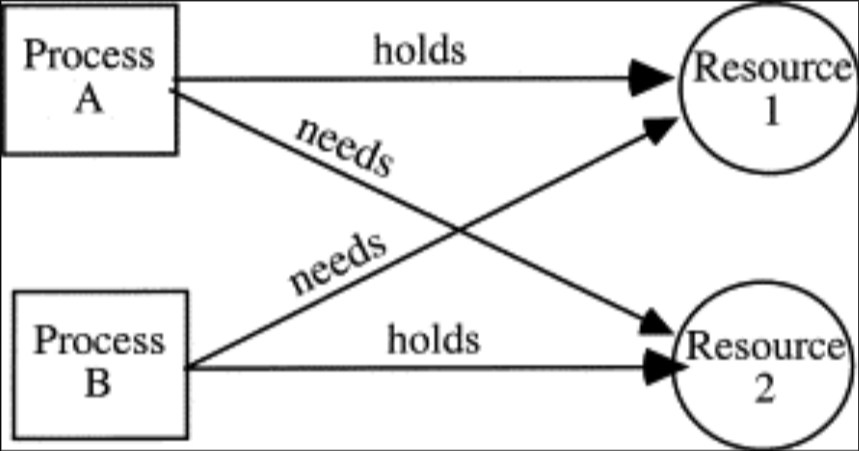
\includegraphics[width=0.5\textwidth]{race.png}} % Espacio para tu captura
\end{frame}

\begin{frame}{Sincronización de procesos: Semáforo Mutex}
    Para evitar condiciones de carrera en el color del LED:
    \begin{itemize}
        \item Se utiliza un \texttt{SemaphoreHandle\_t} de tipo \textbf{Mutex}.
        \item \textbf{TASK A} toma el mutex antes de leer el color para el parpadeo.
        \item \textbf{Timer Callback} toma el mutex antes de actualizar el color global.
    \end{itemize}
    \begin{block}{Teorema}
        El mutex se libera inmediatamente después de la operación crítica para no bloquear el sistema.
    \end{block}
\end{frame}

\begin{frame}[fragile]{Sincronización de procesos: Semáforo Mutex}
  \textbf{TASK A} toma el mutex, realiza la operación crítica (parpadeo), y luego lo libera:
\begin{lstlisting}[language=C]
    while (1) {
        // tomo control del mutex
        if (xSemaphoreTake(params->color_mutex, pdMS_TO_TICKS(500)) == pdTRUE) {
        // ... 
          xSemaphoreGive(params->color_mutex);         
        }
        // espera activa (busy waiting) si no pudo tomar el mutex
        vTaskDelay(pdMS_TO_TICKS(100));
    }
\end{lstlisting}
\end{frame}

\begin{frame}{Sincronización de procesos: Exclusión mutua}
  Exclusión mutua mediante el uso de regiones críticas:

  \vspace{3mm}
\centering
\fbox{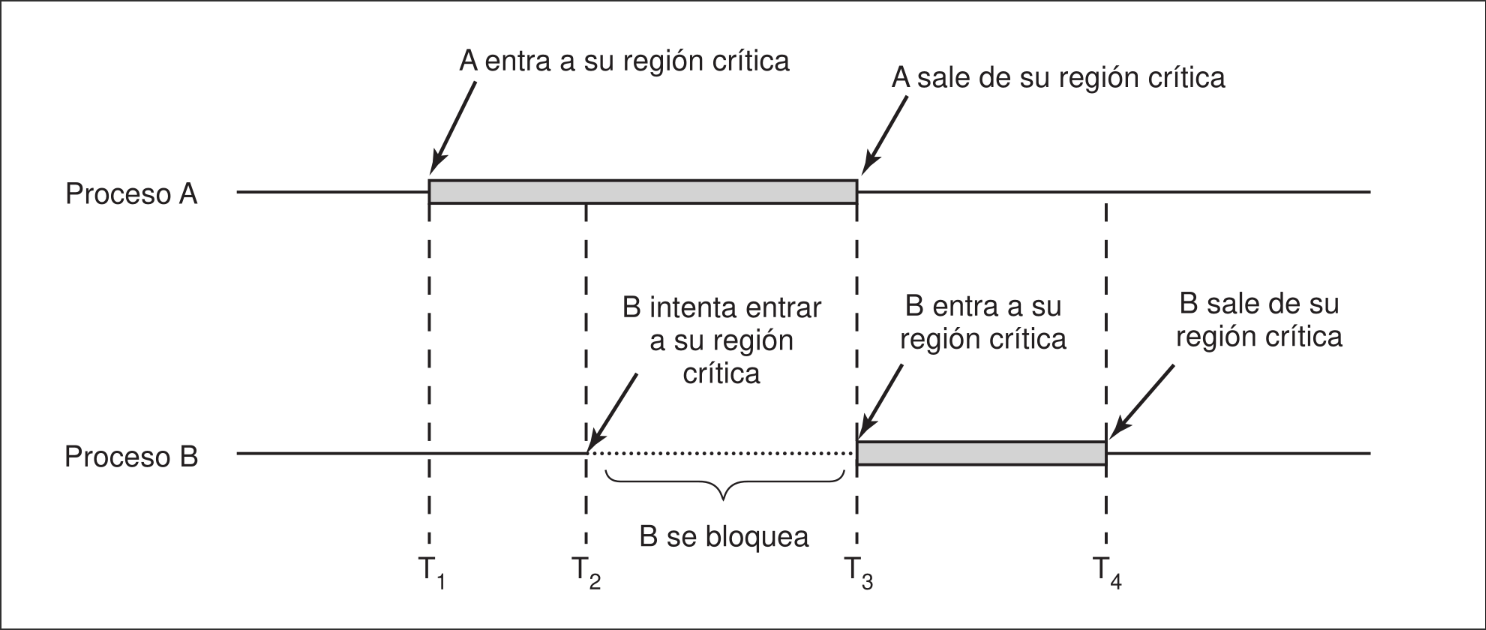
\includegraphics[width=0.8\textwidth]{mutex.png}} % Espacio para tu captura


  \vspace{3mm}
  Extraido de Tanenbaum, 2009.
\end{frame}


\section{Comunicación entre procesos: Colas}

\begin{frame}[fragile]{Comunicación entre procesos: Colas}

La comunicación entre \textbf{TASK\_B} y \textbf{TASK\_C} se realiza mediante una 
\texttt{Queue} de FreeRTOS.

\vspace{0.3cm}

\textbf{TASK\_B} recibe comandos desde UART y los encola:

\begin{lstlisting}[language=C]
led_command_t cmd;
cmd.color = color;
cmd.delay_s = delay_s;

xQueueSend(queue, &cmd, pdMS_TO_TICKS(100));
\end{lstlisting}

\vspace{0.2cm}

\textbf{TASK\_C} permanece bloqueada esperando comandos:

\begin{lstlisting}[language=C]
led_command_t cmd;
while (1) {
    if (xQueueReceive(queue, &cmd, portMAX_DELAY) == pdTRUE) {
        // crear timer y aplicar color
    }
}
\end{lstlisting}



\end{frame}

\begin{frame}[fragile]{Flujo General de TASK\_B (Recepción UART)}
    \begin{columns}[T] % Alineación superior de las columnas
        
        % --- COLUMNA IZQUIERDA: LECTURA Y PARSEO ---
        \begin{column}{0.48\textwidth}
            \textbf{1. Captura de Bytes Bloqueante}
            \begin{itemize}
                \item Espera en buffer sin consumo de CPU.
                \item Acumula caracteres secuencialmente hasta detectar fin de línea (\texttt{\textbackslash n} o \texttt{\textbackslash r}).
            \end{itemize}
            \begin{lstlisting}[basicstyle=\ttfamily\tiny]
int n = uart_read_bytes(UART_NUM_0, &byte, 1, portMAX_DELAY);
            \end{lstlisting}
            
            \vspace{0.2cm}
            \textbf{2. Validación de Formato (Parsing)}
            \begin{itemize}
                \item Extrae campos mediante patrones.
                \item Si falla la estructura \texttt{<COLOR> <SEGUNDOS>}, descarta con \texttt{ESP\_LOGW}.
            \end{itemize}
            \begin{lstlisting}[basicstyle=\ttfamily\tiny]
if (sscanf(line, "%15s %u", color_str, &delay_s) != 2)
            \end{lstlisting}
        \end{column}
        
        % --- COLUMNA DERECHA: TRADUCCIÓN Y ENCOLADO ---
        \begin{column}{0.48\textwidth}
            \textbf{3. Traducción a Diccionario RGB}
            \begin{itemize}
                \item Mapea cadenas de texto (\textit{rojo, verde, azul...}) a estructuras discretas \texttt{color\_t}.
            \end{itemize}
            \begin{lstlisting}[basicstyle=\ttfamily\tiny]
if (!parse_color(color_str, &cmd.color))
            \end{lstlisting}
            
            \vspace{0.2cm}
            \textbf{4. Intercomunicación y Confirmación}
            \begin{itemize}
                \item \textbf{Encolado} Envía el comando estructurado con un timeout de 100~ms para evitar bloqueos por cola llena.
            \end{itemize}
            \begin{lstlisting}[basicstyle=\ttfamily\tiny]
if (xQueueSend(queue, &cmd, pdMS_TO_TICKS(100)) == pdPASS) {
    snprintf(ack, sizeof(ack), "OK: %s\n", color_str);
    uart_write_bytes(UART_NUM_0, ack, strlen(ack));
}
            \end{lstlisting}
        \end{column}

    \end{columns}
    
    \vfill
\end{frame}

% --- SECCIÓN: TIMER Y MEMORIA ---
\section{Gestión de Timers}

% --- SECCIÓN: TASK C ---
\begin{frame}{TASK C: rol dentro del sistema}
    \begin{block}{Responsabilidad principal}
        \textbf{TASK C} recibe comandos desde la cola y programa la aplicación futura del color mediante un \textbf{software timer}.
    \end{block}

    \begin{itemize}
        \item Recibe estructuras de tipo \texttt{led\_command\_t}.
        \item Cada comando contiene:
        \begin{itemize}
            \item un color RGB;
            \item un retardo en segundos.
        \end{itemize}
        \item No prende ni apaga directamente el LED físico.
        \item Su función es actualizar, en el momento correcto, la variable compartida \texttt{current\_color}.
    \end{itemize}

    \vfill
    \centering
    \textit{TASK C funciona como intermediaria entre el comando recibido y el cambio efectivo de color.}
\end{frame}

\begin{frame}[fragile]{Flujo interno de TASK C}
    \begin{columns}
        \begin{column}{0.55\textwidth}
            \begin{enumerate}
                \item Espera comandos en la cola.
                \item Al recibir uno, reserva memoria para el color.
                \item Convierte segundos a ticks.
                \item Crea un timer \textit{one-shot}.
                \item Inicia el timer.
                \item Vuelve a esperar nuevos comandos.
            \end{enumerate}
        \end{column}

        \begin{column}{0.45\textwidth}
\begin{verbatim}
TASK_C
  v
xQueueReceive()
  v
pvPortMalloc()
  v
xTimerCreate()
  v
xTimerStart()
  v
espera otro comando
\end{verbatim}
        \end{column}
    \end{columns}

    \vspace{2mm}

    \begin{block}{Ojaldre}
        TASK C \textbf{no espera bloqueada} el delay del comando. Crea un timer y queda disponible para procesar otros comandos.
    \end{block}
\end{frame}

\begin{frame}[fragile]{Timer callback: aplicación del color}
Cuando vence el timer, FreeRTOS ejecuta automáticamente el callback:

\begin{lstlisting}
static void color_timer_callback(TimerHandle_t xTimer) {
    color_t *new_color =
        (color_t *) pvTimerGetTimerID(xTimer);

    if (xSemaphoreTake(s_color_mutex,
                       portMAX_DELAY) == pdTRUE) {
        s_current_color->r = new_color->r;
        s_current_color->g = new_color->g;
        s_current_color->b = new_color->b;

        xSemaphoreGive(s_color_mutex);
    }

    vPortFree(new_color);
    xTimerDelete(xTimer, 0);
}
\end{lstlisting}
\end{frame}

\begin{frame}{Timer callback: puntos clave}
    \begin{itemize}
        \item El callback \textbf{no se llama manualmente}: lo ejecuta FreeRTOS cuando vence el timer.
        \item Recupera el color asociado al timer con \texttt{pvTimerGetTimerID()}.
        \item Toma el mutex para modificar \texttt{current\_color}.
        \item Libera el mutex después de la operación crítica.
        \item Libera la memoria dinámica con \texttt{vPortFree()}.
        \item Elimina el timer con \texttt{xTimerDelete()}.
    \end{itemize}

    \begin{block}{Resumen}
        TASK C programa la acción; el callback ejecuta el cambio real del color.
    \end{block}
\end{frame}
\section{Punto de entrada (Main)}

\begin{frame}[fragile]{Punto de entrada: Creación de tareas}
  Según la API de FreeRTOS:
  \begin{lstlisting}[language=C]
 BaseType_t xTaskCreate( TaskFunction_t pvTaskCode,
                         const char * const pcName,
                         const configSTACK_DEPTH_TYPE uxStackDepth,
                         void *pvParameters,
                         UBaseType_t uxPriority,
                         TaskHandle_t *pxCreatedTask
                       );
\end{lstlisting}
Ejemplo de creación de \textbf{TASK B}:
\begin{lstlisting}[language=C]
static task_b_params_t task_b_params;
task_b_params.command_queue = command_queue;
xTaskCreate(task_b, "TASK_B", CONFIG_ESP32_PTHREAD_TASK_STACK_SIZE_DEFAULT, &task_b_params, task_b_prio,
            &task_b_handler);
\end{lstlisting}
\end{frame}

% --- SECCIÓN: LOGS Y RESULTADOS ---
\section{Resultados}

\begin{frame}{Trazabilidad y Logs}
    Uso de macros \texttt{ESP\_LOG}:
    \begin{itemize}
        \item \textbf{INFO (ESP\_LOGI)}: Ej: Comando recibido.
        \item \textbf{WARN (ESP\_LOGW)}: \texttt{TASK B: unknown color: 'tiza'}.
        \item \textbf{ERROR (ESP\_LOGE)}: Errores fatales.
    \end{itemize}
    Ejemplo de logs:

    \centering
    \fbox{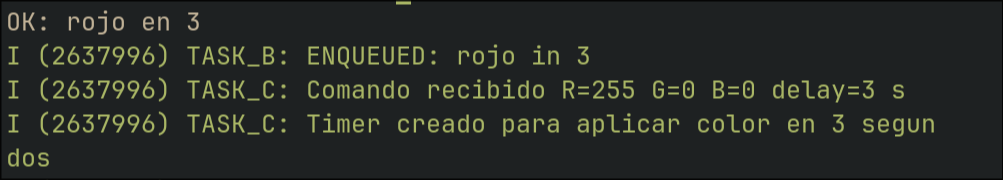
\includegraphics[width=0.9\textwidth]{logi.png}} % Espacio para tu captura

    \centering
    \fbox{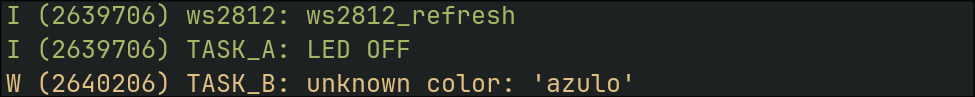
\includegraphics[width=0.9\textwidth]{logw.png}} % Espacio para tu captura
\end{frame}


\section{Conclusiones}

\begin{frame}{Flujo general del proyecto}
    \centering

    \resizebox{0.96\textwidth}{!}{
    \begin{tikzpicture}[
        box/.style={
            rectangle,
            rounded corners,
            draw=UCUBlue,
            thick,
            align=center,
            minimum width=2.45cm,
            minimum height=1cm,
            fill=UCUBlue!8,
            font=\scriptsize
        },
        arrow/.style={-{Latex[length=2mm]}, thick, UCUBlue},
        node distance=1.1cm and 0.8cm
    ]

    % Fila superior
    \node[box] (uart) {Usuario\\\texttt{azul 2}};
    \node[box, right=of uart] (taskb) {\textbf{TASK B}\\UART + parsing\\prioridad alta};
    \node[box, right=of taskb] (queue) {\textbf{Queue}\\\texttt{led\_command\_t}};
    \node[box, right=of queue] (taskc) {\textbf{TASK C}\\recibe comando\\crea timer};

    % Fila inferior
    \node[box, below=1.25cm of taskc] (timer) {\textbf{Software Timer}\\one-shot};
    \node[box, left=of timer] (callback) {\textbf{Callback}\\toma mutex\\actualiza color};
    \node[box, left=of callback] (color) {\textbf{current\_color}\\recurso compartido};
    \node[box, left=of color] (taska) {\textbf{TASK A}\\lee color\\parpadea LED};

    % Flechas
    \draw[arrow] (uart) -- (taskb);
    \draw[arrow] (taskb) -- node[above, font=\tiny]{\texttt{xQueueSend()}} (queue);
    \draw[arrow] (queue) -- node[above, font=\tiny]{\texttt{xQueueReceive()}} (taskc);
    \draw[arrow] (taskc) -- node[right, font=\tiny]{\texttt{xTimerCreate()}} (timer);
    \draw[arrow] (timer) -- node[below, font=\tiny]{vence} (callback);
    \draw[arrow] (callback) -- node[below, font=\tiny]{mutex} (color);
    \draw[arrow] (color) -- node[below, font=\tiny]{lee} (taska);

    \end{tikzpicture}
    }

    \vspace{3mm}

    \begin{block}{Resumen}
        \texttt{TASK B} recibe el comando; \texttt{TASK C} programa cuándo aplicarlo;
        el callback actualiza \texttt{current\_color}; y \texttt{TASK A} refleja ese color en el LED.
    \end{block}
\end{frame}

% --- CONCLUSIÓN ---
\begin{frame}{Bibliografía}
\begin{itemize}
    \item Tanenbaum, A. S. (2009). \textit{Sistemas Operativos Modernos} (3.ª ed.). Pearson Educación.
    \item Silberschatz, A., Galvin, P. B., \& Gagne, G. (2018). \textit{Operating System Concepts} (10th ed.). Wiley.
    \item Real Time Engineers Ltd. (s. f.). \textit{FreeRTOS Reference Manual}. Recuperado de \url{https://www.freertos.org/Documentation/}
\end{itemize}
\end{frame}

% Slide Final
\begin{frame}
    \centering
    \Huge \textcolor{UCUBlue}{¿Preguntas?}
    \vfill
    \normalsize \insertauthor \\ 
    \vspace{5mm}
    \insertinstitute
\end{frame}

\end{document}
